\documentclass[12pt,a4paper]{article}

\usepackage{epcc}
\usepackage{graphics}
\usepackage{epigraph}

\setlength\epigraphwidth{.8\textwidth}
\setlength\epigraphrule{0pt}
% This example file shows how a thesis can be laid out using Latex. It
% does not use any special local features so should be portable to other
% places.
%
% To produce myfile.pdf from myfile.tex type:
% 
% pdflatex myfile
%
% Note that pdflatex expects all included figures to be in PDF too. See
% the includegraphics command below.


% This document contains many cross-references and forward references,
% eg in constructing a table of contents, so Latex may need to be run
% twice to get all the references correct. If you need to run Latex twice
% you may get the warning:
% 
% LaTeX Warning: Label(s) may have changed. Rerun to get cross-references right


\begin{document}

\title{Modelling Room Acoustics with a GPU}
\author{Jacob Josiah Webber}
\date{18 August 2017}

\makeEPCCtitle

\thispagestyle{empty}

\newpage

\pagenumbering{roman}

\tableofcontents

\newpage

\section*{Acknowledgements}

Many thanks to all who helped me with this dissertation.

\section*{Note}

This is my work I am no a cheat.



\newpage
\pagenumbering{arabic}

\section{Introduction}
\epigraph{\itshape ``There is no competition of sounds between a nightingale and a violin.''}{Dejan Stojanovic}

The way we perceive sound depends on the environment in which we hear it as well as how the sound was created. Listening to a sound in a space like a church or a cathedral is very different to listening in a bedroom. Being able to predict how a space will affect a sound has practical use in the design of new spaces, particularly those spaces where acoustic performance is critical. A great deal of effort goes into the design of new concert halls. This would be greatly enhanced by accurate acoustic models of spaces. The aim then, of research in this area, is to provide an accurate prediction of how a space will sound after being given its physical properties.

The key technique currently used for these simulations is the finite-difference time-domain (FDTD) method for finding approximate solutions to the wave equation across a three dimensional space. This forms a simple stencil. This stencil process across a vast number of points in memory is well suited to the use of graphics processing units (GPUs) which have high band width graphics memory and can operate on very many points in a massively parallel fashion.

In the work leading up to this report, a novel technique was devised and implemented that performs these simulations. This approach was designed to make best use of graphics memory, which is relatively scarce.

\newpage
\section{Background and Literature Review}

\epigraph{\itshape ``He who loves practice without theory is like the sailor who boards ship without a rudder and compass and never knows where he may cast.''}{Leonardo da Vinci}

\subsection{Room Acoustics}

Sound is modelled using the wave equation.

\begin{displaymath}
E=mc^{2}
\end{displaymath}

\subsection{Graphics Processing Units (GPUs)}

\subsection{The Proposed Data Structure and Method}
% note that labels do not need to include a description of the object
% they are labelling but it can be helpful, eg \label{fig:figurename}.

You can use a label on a figure to refer to it later. The university
crest is in \ref{fig:eucrest}. Note that you should not use phrases like
``the figure above'' or ``the following figure'' since Latex may move
the figure relative to the text if it cannot be fitted onto the current page.

\subsection{Possible Spectral Techniques}
While no work was done on this, I am going to talk about it anyway.

\newpage
\section{Design and Implementation}
\epigraph{\itshape ``The first 90 percent of the code accounts for the first 90 percent of the development time...The remaining 10 percent of the code accounts for the other 90 percent of the development time.''}{Tom Cargill}

\subsection{Software Development Process}

\subsection{Debugging and Profiling Tools}

\newpage
\section{Results and Analysis}

\subsection{Some results}
Here are some results.

\subsubsection{More results}
When showing results you are likely to use tables and graphs. You can
create tables easily in Latex.

\begin{table}[h]
\begin{center}
\begin{tabular}{||l|c|l||}
\hline
{\bf File names} & {\bf Satellite} & {\bf Resolution}\\
\hline
  worldr         &  Meteosat     &   5km\\
  worldg         &  Meteosat     &   5km\\
  worldb         &  Meteosat     &   5km\\
\hline
\end{tabular}
\end{center}
\caption{This is a simple table. More complicated tables can have
headings which pass over more than one column}
\label{simple_table}
\end{table}

If you want to produce fancier tables than shown in Table \ref{simple_table}
refer to the manual.

\subsubsection{Graphs}

Perhaps the most robust way to include graphs is to create then using
whatever package you like (eg Excel, gnuplot, xmgrace, ...) and then
convert them to PDF and include them in the same was as was done in
Figure~\ref{fig:eucrest} for the University Crest. Nowadays you can
usually do this with most packages including Microsoft ones.

\begin{figure}[h]
\begin{center}
\resizebox{0.75\hsize}{!}{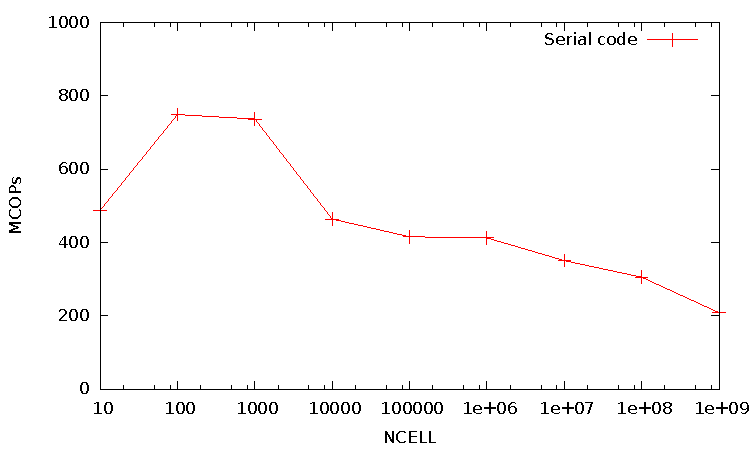
\includegraphics{serialscale}}
\caption{Simple gnuplot example: performance of traffic model}
\label{fig:gnu}
\end{center}
\end{figure}

You can produce the PDF version of Figure~\ref{fig:gnu} from the file
\texttt{serialscale.gp} using \texttt{gnuplot serialscale.gp}.

\section{Conclusions}

This is the place to put your conclusions about your work.

\begin{thebibliography}{100}

\bibitem{ref:lam} L.Lamport. {\em 1986 Latex User's Guide
and Reference Manual.} Addison Wesley. pp242.

\bibitem{ref:bloggs} F.Bloggs. {\em 1993 Latex Users do it
in Environments} Int. Journal of Silly Findings. pp 23-29.

\end{thebibliography}


\end{document}

